% !TeX spellcheck = nb_NO
% Kommentaren ovenfor gir instruks til editoren din om at den skal bruke norsk stavekontroll. Dette fungerer bl.a. i TeXstudio.

\documentclass[a4paper,norsk]{article}
% Norsk orddeling
\usepackage[norsk]{babel}
% AMS-pakkene er nyttige
\usepackage{amsmath,amsfonts,amssymb,amsthm}
% For å definere lister, som f.eks. deloppgaver
\usepackage{enumitem}
% Inneholder mye nyttig, slik som \coloneqq
\usepackage{mathtools}
% Penere kalligrafiske fonter
\usepackage[utf8]{inputenc}
\usepackage[T1]{fontenc}
\usepackage[a4paper, margin=0.5in]{geometry}
\usepackage{mathabx}
\usepackage{listings}
\usepackage{xcolor}
\usepackage{ifthen}

\usepackage[most]{tcolorbox}
\tcbuselibrary{theorems, breakable, skins}
\tcbset{before upper=\par, after upper=\par} % allows itemize and enumerate inside boxes

\usepackage{hyperref}



\tcbset{
  % Better page breaking for all tcolorbox environments
  enhanced,
  breakable,
  before skip=5pt plus 2pt minus 1pt,
  after skip=5pt plus 2pt minus 1pt,
  parbox=false,
}
\newtcbtheorem[]{definitionbox}{Definisjon}{
  colback=blue!3,
  colframe=blue!70!black,
  fonttitle=\bfseries\color{white},
  coltitle=white,
  boxrule=0.6pt,
  arc=2mm,
  enhanced,
  breakable
}{def}

\newtcbtheorem[]{theorembox}{Teorem}{
  colback=green!3,
  colframe=green!50!black,
  fonttitle=\bfseries,
  coltitle=black,
  boxrule=0.6pt,
  before upper=\par\ignorespaces,
  after upper=\par\unskip,
  arc=2mm,
  enhanced,
  breakable
}{thm}

\newtcbtheorem[]{oppgavebox}{Oppgave}{
  colback=gray!5,
  colframe=black!60,
  fonttitle=\bfseries,
  coltitle=black,
  boxrule=0.6pt,
  arc=2mm,
  enhanced,
  breakable,
  parbox=false
}{oppg}

\newtcolorbox{sectionbox}[1][]{
  colback=white,
  colframe=black!70,
  boxrule=0.7pt,
  arc=3mm,
  top=2mm, bottom=2mm, left=2mm, right=2mm,
  title=#1,
  enhanced,
  breakable
}

\newtcbtheorem[]{corollarybox}{Korollar}{
  colback=purple!5,
  colframe=purple!60!black,
  fonttitle=\bfseries\color{white},
  coltitle=white,
  boxrule=0.6pt,
  arc=2mm,
  enhanced,
  breakable,
  before upper=\par\ignorespaces,
  after upper=\par\unskip
}{cor}

\newtcbtheorem[]{lemmabox}{Lemma}{
  colback=orange!5,
  colframe=orange!70!black,
  fonttitle=\bfseries,
  boxrule=0.6pt,
  arc=2mm,
  enhanced,
  breakable
}{lem}

\newtcbtheorem[]{propositionbox}{Proposisjon}{
  colback=cyan!5,
  colframe=cyan!60!black,
  fonttitle=\bfseries,
  coltitle=black,
  boxrule=0.6pt,
  arc=2mm,
  enhanced,
  breakable
}{prop}

\newtcbtheorem[]{proofbox}{Bevis}{
  enhanced,
  breakable,
  colback=white,
  colframe=black,
  fonttitle=\bfseries\color{white},
  coltitle=white,
  colbacktitle=black,
  title style={opacity=0.9},
  boxrule=0.6pt,
  arc=2mm,
  before upper=\par\ignorespaces,
  after upper=\par\unskip,
  parbox=false, % Viktig for sidebryting
  segmentation style={black,solid,opacity=0.2,line width=0.5pt}
}{proof}

\newlist{suboppgave}{enumerate}{1}
\setlist[suboppgave,1]{
  label=\textbf{(\alph*)},
  ref=\theenumi\alph*,
  leftmargin=1.5em,
  itemsep=0.4em,
  topsep=0.3em,
  parsep=0pt,
  partopsep=0pt
}



\setcounter{secnumdepth}{2}  % Sections and subsections numbered

% Python style  
\lstdefinestyle{pythonstyle}{
    language=Python,
    basicstyle=\ttfamily\small,
    keywordstyle=\color{blue},
    commentstyle=\color{green},
    numbers=left,
    frame=single
}

% Bruk bedre symboler for ≥, ≤, epsilon og phi
\renewcommand{\geq}{\geqslant}
\renewcommand{\leq}{\leqslant}
\newcommand{\eps} {\varepsilon}
\renewcommand{\epsilon}{\varepsilon}
\renewcommand{\phi}{\varphi}

% Definer de vanligste mengdene og funksjonene
\newcommand{\R}{\mathbb{R}}
\newcommand{\K}{\mathbb{K}}
\newcommand{\C}{\mathbb{C}}
\newcommand{\N}{\mathbb{N}}
\newcommand{\Z}{\mathbb{Z}}
\newcommand{\Q}{\mathbb{Q}}
% \L er definert som noe annet fra før av, så vi må redefinere \L
\renewcommand{\L}{\mathcal{L}}
% Rommet av polynomer
\newcommand{\Pol}{{\mathcal{P}}}
\DeclareMathOperator{\id}{id}
\DeclareMathOperator{\Image}{im}
\DeclareMathOperator{\Kernel}{ker}
\DeclareMathOperator{\Span}{span}
\DeclareMathOperator{\Rank}{rank}
\DeclareMathOperator{\Diag}{diag}
\DeclareMathOperator{\Proj}{proj}
\newcommand{\basis}{{\mathcal{B}}}
\newcommand{\basiss}{{\mathcal{C}}}
\newcommand{\basisss}{{\mathcal{D}}}

\newtcolorbox{algoritme}[1]{
  title=Algoritme~#1,
  colback=white,
  colframe=black,
  boxrule=0.5pt,
  arc=2mm,
  left=3mm,
  right=3mm,
  top=1mm,
  bottom=1mm
}

% Definer oppgavemiljøet
\newenvironment{oppgave}[1]%
	{\trivlist{}\item\relax\textbf{Løsning på #1.}\medspace}%
	{\endtrivlist}
% Deloppgavelister
\newlist{deloppgave}{enumerate}{1}
\setlist[deloppgave,1]{label=(\textbf{\alph*}),align=left}

\title{Oblig 4 \\ MAT1125, høst 2025}
\author{Oliver Ekeberg}

\begin{document}
\tableofcontents

\section*{4.1 Indreprodukter}
\addcontentsline{toc}{section}{Indreprodukter}

\begin{definitionbox}{4.1.1}{}
La U være et vektorrom over $ \mathbb{K} $. Et \textbf{\textit{indreprodukt}} på U er en funksjon $ \langle \cdot, \cdot \rangle_{  }: U \times U \to \mathbb{K} $ slik at for alle $ u, v, w \in U $ og $ \alpha_{}^{} \in \mathbb{K} $ er
\begin{itemize}
    \item $ \langle u, u \rangle_{  } \geq 0 $ og $ \langle u, u \rangle_{  } =0 \iff u =0 $
    \item $ \langle u + v, w \rangle_{  } = \langle u, w \rangle_{  } + \langle v, w \rangle_{  }  $
    \item $ \langle \alpha_{}^{} u, v \rangle_{  } = \alpha_{}^{} \langle u, v \rangle_{  } $
    \item $ \langle u, v \rangle_{  } = \overline{ \langle v, u \rangle_{  } } $     
\end{itemize}
Et vektorrom som er utstyrt med et indreprodukt kalles et \textbf{\textit{indreproduktrom}} 
\end{definitionbox}

Dette er en meget viktig egenskap, som kommer inn når man studerer Hilbert rom. Hilbert rom er komplette indreproduktrom

\begin{oppgavebox}{4.1.2}{}
Bevis følgende:
\begin{itemize}
    \item a) Indreproduktet er additivt i andre argument $ \langle u, v + w \rangle_{  } = \langle u, v \rangle_{  } + \langle u, w \rangle_{  }  $ 
    \item b) Indreproduktet er konjugert-homogen i andre argument $ \langle u, \alpha_{}^{} v \rangle_{  } = \overline{\alpha_{}^{} } \langle u, v \rangle_{  }  $ 
    \item c) Hvis $ \mathbb{K}=\mathbb{R} $ er indreproduktet symmetrisk $ \langle u, v \rangle_{  } = \langle v, u \rangle_{  }  $ 
\end{itemize}

\begin{proofbox}{4.1.2 a)}{}
\begin{align*}
    \langle u, v+ w \rangle_{  } &= \overline{ \langle v+w, u \rangle_{  } } \\
    &= \overline{ \langle v, u \rangle_{  }  + \langle w, u \rangle_{  } }\\
    &= \langle u, v \rangle_{  } + \langle u, w \rangle_{  } 
\end{align*}
\end{proofbox}

\begin{proofbox}{4.1.2 b)}{}
\begin{align*}
    \langle u, \alpha_{}^{} v \rangle_{  } &= \overline{ \langle \alpha_{}^{} v, u \rangle_{  } } \\
    &= \overline{ \alpha_{}^{}  \langle v, u \rangle_{  } } \\
    &= \overline{\alpha_{}^{} } \overline{ \overline{ \langle u, v \rangle_{  } }} \\
    &= \overline{\alpha_{}^{} } \langle u, v \rangle_{  } 
\end{align*}
\end{proofbox}

\begin{proofbox}{4.1.2 c)}{}
Om $ \mathbb{K} = \mathbb{R} $ så er indreproduktet om $ x, y \in R $ lik
\begin{align*}
    \langle x,y \rangle_{  } &= x^T\cdot y\\
    &= \sum_{ j=1 }^{ n } x_j \cdot y_j \\
    &= \sum_{ j=1 }^{ n } y_j \cdot x_j \\
    &= y^T \cdot x \\
    &= \langle y, x \rangle_{  } 
\end{align*}
\end{proofbox}
\end{oppgavebox}

\begin{oppgavebox}{4.1.3}{}
La $ u \in U $ være slik at $ \langle u, v \rangle_{  } = 0 \; \forall v \in U $. Vis at $ u=0 $. Er det samme sant hvis $ \langle v, u \rangle_{  } = 0 \; \forall v \in U $? 
\begin{proofbox}{4.1.3}{}
Vet at $ u \in U $ og at $ \langle u, v \rangle =0 $ for den utvalgte u $ \forall v \in U $. Skal først vise at $ u=0 $.

$ \forall v \in U$, $ \exists u \in U $ s.a. $ v=u $. Siden $ \langle u, v \rangle =0 \forall v \in U $, så må $ \langle u,u \rangle = 0$. Fra første egenskap av indreproduktrom vet vi at
\[
    \langle u, u \rangle =0 \Longleftrightarrow u=0
\]
Og vi har vist at $ u=0 $. Spørsmålet er nå om det samme gjelder dersom $ \langle v, u \rangle =0 $ for alle $ v \in U $.
\[
    \langle v, u \rangle = \overline{ \langle u, v \rangle }
\]
Siden $ 0 = \overline{0} $ , så er $ \langle v, u \rangle = \overline{0}  =0$. Det kommer av at $ \langle u, v \rangle =0 $ som vi allerede har vist
\end{proofbox}
\end{oppgavebox}


\begin{definitionbox}{4.1.4}{}
La U være et indreproduktrom. Vi sier at $ u, v \in U $ er \textbf{\textit{ortogonale}}, og skriver $ u \bot v $, dersom $ \langle u, v \rangle_{  } =0 $ 
\end{definitionbox}



\begin{oppgavebox}{4.1.5}{}

\begin{proofbox}{4.1.5 a)}{}
    Vi har det kanoniske prikkproduktet for $ \mathbb{K}^n $ 

    \[
        \langle x, y \rangle _{\mathbb{K}^n} := x^T \overline{y} = \sum_{ k=1 }^{ n } x_k \overline{y}_k
    \]

    Skal nå vise at det er et prikkprodukt. Da må det tilfredsstille i)-iv)

    \begin{enumerate}
        \item \[
            \langle x, x \rangle = x^T \overline{x} = \sum_{ k=1 }^{ n } x_k \overline{x}_k  
        \]
         
        som er $ \geq 0 $ og $ =0 \Longleftrightarrow x=0$  
        \item for en $ z \in \mathbb{K}^n $ er  \[
            \langle x+y, z \rangle = \sum_{ k=1 }^{ n } (x+y)_k \overline{z}_k 
            = \sum_{ k=1 }^{ n } x_k \overline{z}_k + y_k \overline{z}_k 
            = \langle x, z \rangle + \langle y, z \rangle 
        \]
        

        \item for en $ a \in \mathbb{K} $ er \[
            \langle ax, y \rangle = \sum_{ k=1 }^{ n } ax_k \overline{y}_k 
            = a \sum_{ k=1 }^{ n } x_k \overline{y}_k 
            = a \langle x, y \rangle 
        \]
        

        \item \[
            \langle x, y \rangle = \sum_{ k=1 }^{ n } x_k \overline{y}_k 
            = \sum_{ k=1 }^{ n } \overline{y}_k x_k
            = \sum_{ k=1 }^{ n } \overline{ y_k \overline{x_k}}
            = \overline{\langle y, x \rangle}  
        \]
    \end{enumerate}
    Og jeg har vist at $ \langle x, y \rangle _{\mathbb{K}^n} $ er et indreproduktrom 
\end{proofbox}

\begin{proofbox}{4.1.5 c)}{}
    Vi har l2 rommet $\ell^2(\mathbb{K}) := 
    \left\{ (a_1, a_2, \ldots) \; : \; 
    \sum_{k \in \mathbb{N}} |a_k|^2 < \infty 
    \right\}$. Vi definerere så $ \ell^2 $ indreproduktet som 

    \[
        \langle a, b \rangle _{\ell^2} := \sum_{ k=1 }^{ \infty } a_k \overline{b}_k
    \]
    Skal nå vise at dette er et indreproduktrom

    \begin{enumerate}
        \item \[
            \langle a, a \rangle _{\ell^2} = \sum_{ k=1 }^{ \infty } a_k \overline{a}_k
        \]
        Og dette er åpenbart $ \geq 0 $ og $ =0 \Longleftrightarrow a_k=0 \forall k=1,2,...$  

        \item for en $ c = \left( c_1, c_2, ... \right) \in \ell^2 (\mathbb{K}) $ så er
        
        \[
            \langle a+b, c \rangle _{\ell^2} = \sum_{ k=1 }^{ \infty } \left( a + b \right) _k \overline{c}_k 
            = \sum_{ k=1 }^{ \infty } \left( a_k + b_k \right) \overline{c}_k 
            = \sum_{ k=1 }^{ \infty } a_k \overline{c}_k + b_k \overline{c}_k 
            = \langle a, c \rangle _{\ell^2} + \langle b, c \rangle _{\ell^2}
        \]
        

        \item for en $ \alpha_{}^{} \in \mathbb{K} $ så er  \[
            \langle \alpha_{}^{} a, b \rangle_{ \ell^2 } = \sum_{ k=1 }^{ \infty } \left( \alpha_{}^{} a \right) _k \overline{b}_k 
            = \sum_{ k=1 }^{ \infty } \alpha_{}^{} a_k \overline{b}_k 
            = \alpha_{}^{} \sum_{ k=1 }^{ \infty } a_k \overline{b}_k 
            = \alpha_{}^{} \langle a, b \rangle_{ \ell^2 } 
        \]
        

        \item \[
            \langle a, b \rangle_{ \ell^2 } = \sum_{ k=1 }^{ \infty } a_k \overline{b}_k 
            = \sum_{ k=1 }^{ \infty } \overline{b}_k a_k 
            = \sum_{ k=1 }^{ \infty } \overline{b_k \overline{a_k}}
            = \overline{ \langle b, a \rangle_{ \ell^2 } }
        \]
        
    \end{enumerate}
\end{proofbox}

\begin{proofbox}{4.1.5 d)}{}
    Vi har $ f, g \in C \left( \left[ a, b \right], \mathbb{K} \right)   $. Vi definererer $ L^2 $ indreproduktet som
    
    \[
        \langle f, g \rangle_{ L^2 } := \int_{a}^{b} f(t) \overline{g(t)} dt
    \]

    \begin{enumerate}
        \item \[
            \langle f, f \rangle_{ L^2 } = \int_{a}^{b} f(t) \overline{f(t)} dt
        \]
        
        Dette er åpenbart $ \geq 0 $ og $ =0 \Longleftrightarrow f(t) = 0 \forall t \in \left[ a, b \right]  $ 
        
        \item for en $ h \in C \left(  \left[ a, b \right] \mathbb{K} \right)  $ så er 
        
        \[
            \langle f+g, h \rangle_{ L^2 } = \int_{a}^{b} (f+g)(t) \overline{h(t)} dt 
            = \int_{a}^{b} f(t) \overline{h(t)} + g(t) \overline{h(t)} dt 
            = \int_{a}^{b} f(t) \overline{h(t)}dt + \int_{a}^{b} g(t) \overline{h(t)}dt \\
            = \langle f, h \rangle_{ L^2 } + \langle g, h \rangle_{ L^2 } 
        \]
        


        \item For en $ \alpha_{}^{} \in \mathbb{K} $ så har vi
        \[
            \langle \alpha_{}^{} f, g \rangle_{ L^2 } = \int_{a}^{b} \left( \alpha_{}^{} f \right)(t) \overline{g(t)}dt 
            =  \int_{a}^{b} \alpha_{}^{} f(t) \overline{g(t)}dt 
            = \alpha_{}^{} \int_{a}^{b} f(t) \overline{g(t)}dt 
            = \alpha_{}^{} \langle f, g \rangle_{ L^2 } 
        \]
        

        \item Vi har her at 
        \[
            \langle f, g \rangle_{L^2} 
                = \int_a^b f(t)\,\overline{g(t)}\,dt 
                = \int_a^b \overline{g(t)}\,f(t)\,dt 
                = \overline{\langle g, f \rangle_{L^2}}
        \]  
        Fordi $ \overline{g} f = \overline{g \overline{f}} $
    \end{enumerate}
\end{proofbox}
\end{oppgavebox}

\section*{4.2 Normen indusert av et indreprodukt}
\addcontentsline{toc}{section}{Normen indusert av et indreprodukt}

\begin{definitionbox}{4.2.1}{}
La U være et normert vektorrom med indreprodukt $ \langle \cdot, \cdot \rangle_{  }  $. \textbf{\textit{Normen indusert av et indreprodukt}} er funksjonen 
\[
    \left\lVert u \right\rVert := \sqrt{ \langle u, u \rangle_{  }  }
\]
for $ u \in U $. Dette er et reelt ikke negativt tall for alle $ u \in  U $. Derfor er uttrykket $ \sqrt{ \langle u, u \rangle_{  }  } $ veldefinert, reelt og ikkenegativt. 
\end{definitionbox}

\begin{oppgavebox}{4.2.2}{}
Vis at $ L^2$-normen  $ \left\lVert f \right\rVert _{L^2} := \left( \int_{a}^{b} \left| f(t) \right| ^2 dt  \right)^{ \frac{ 1 }{ 2 }}  $  er normen indusert av indreproduktet $ \langle f, g \rangle_{ L^2 } := \int_{a}^{b} f(t) \overline{g(t)} dt  $ 

\begin{proofbox}{4.2.2}{}
Vi har at 
\[
    \langle f, f \rangle_{ L^2 } = \int_{a}^{b} f(t) \overline{f(t)}dt = \int_{a}^{b} \left| f(t) \right| ^2    dt  
\]
Da vil 
\[
    \left\lVert f \right\rVert _{ L^2} = \left( \langle f, f \rangle_{ L^2 }  \right) ^{ \frac{ 1 }{ 2 }} = \left( \int_{a}^{b} \left| f(t) \right| ^2    dt  \right) ^{ \frac{ 1 }{ 2 }}
\]



\end{proofbox}
\end{oppgavebox}

\begin{propositionbox}{4.2.3}{}
Normen indusert av indreprodukt er en norm
\end{propositionbox}

Før vi beviser 4.2.3 ser på teoremet her
\begin{theorembox}{Cauchy-Schwartz ulikheten}{}
La $ \left\lVert \cdot  \right\rVert  $ være normen indusert av et indreprodukt $ \langle \cdot, \cdot   \rangle_{  }  $. Da er
\[
    \left| \langle u, v \rangle_{  }  \right| \leq \left\lVert u \right\rVert ^2 \left\lVert v \right\rVert ^2
\]


\end{theorembox}

\begin{proofbox}{4.2.3}{}
    Hvis u eller v er lik 0, er begge sider lik 0. Anta derfor at både u og v er ulik 0. Vi får da

\[
    0 \leq \left\lVert u - \frac{ \langle u, v \rangle_{  }  }{ \left\lVert v \right\rVert ^2 } v \right\rVert ^2 = \langle u - \frac{ \langle u, v \rangle_{  }  }{ \left\lVert v \right\rVert ^2 } v, u - \frac{ \langle u, v \rangle_{  }  }{ \left\lVert v \right\rVert ^2 } v  \rangle_{  } 
\]
\[
    = \langle u, u \rangle_{  } - \frac{ \overline{ \langle u, v \rangle_{  } } }{ \left\lVert v \right\rVert ^2 } \langle u, v \rangle_{  } - \frac{ \langle u, v \rangle_{  }  }{ \left\lVert v \right\rVert ^2 } \langle v, u \rangle_{  } + \frac{ \left| \langle u, v \rangle_{  }  \right| ^2 }{ \left\lVert v \right\rVert ^4 } \langle v, v \rangle_{  } = \left\lVert u \right\rVert ^2 - \frac{ 2 \left| \langle u, v \rangle_{  }  \right| ^2 }{ \left\lVert v \right\rVert^2  } + \frac{ \left| \langle u, v \rangle_{  }  \right|^2  }{ \left\lVert v \right\rVert^2  } = \left\lVert u \right\rVert ^2 - \frac{ \left| \langle u, v \rangle_{  }  \right|^2  }{ \left\lVert v \right\rVert ^2 }
\]
Stokker vi om får vi at
\[
    \left| \langle u, v \rangle_{  }  \right|^2 \leq \left\lVert u \right\rVert ^2 \left\lVert v \right\rVert ^2 
\]
\end{proofbox}

\begin{proofbox}{4.2.2}{}
Skal vise at normen indusert av indreprodukt er en norm. begynner med i)
\[
    \left\lVert u \right\rVert ^2 = \langle u, u \rangle_{  } \geq 0
\]
som vi har vist tidligere\\
Viser nå ii) av definijson 3.1.1    
\[
    \left\lVert \alpha_{}^{} u \right\rVert ^2 = \langle \alpha_{}^{} u , \alpha_{}^{}  u \rangle_{  } = \alpha_{}^{} \langle u, \alpha_{}^{} u \rangle_{  } = \alpha_{}^{} \overline{ \langle \alpha_{}^{} u, u \rangle_{  } } = \alpha_{}^{}  \overline{ \alpha_{}^{} } \langle u, u \rangle_{  } = \left| \alpha_{}^{}  \right| ^2 \left\lVert u \right\rVert ^2
\]
\end{proofbox}

\begin{theorembox}{4.2.5 Pythagoras setning}{}
Hvis $ u \bot v $ så er
\[
    \left\lVert u + v \right\rVert ^2 = \left\lVert u \right\rVert ^2 + \left\lVert v \right\rVert ^2
\]
\begin{proofbox}{4.2.5}{}
Siden $ u \bot v $ så er $ \langle u, v \rangle_{  } =0 $  og $ \langle v, u \rangle_{  }  =0$. så
\[
    \left\lVert u+v \right\rVert ^2 = \langle u+v, u+v \rangle_{  } = \left\lVert u \right\rVert ^2 + \langle u, v \rangle_{  } + \langle v, u \rangle_{  } + \left\lVert v \right\rVert ^2 = \left\lVert u \right\rVert ^2 + \left\lVert v \right\rVert ^2
\]
\end{proofbox}
\end{theorembox}

\section*{4.3 Ortogonal og ortonormal liste}
\addcontentsline{toc}{section}{Ortogonal og ortonormal liste}

\begin{definitionbox}{4.3.1}{}
La U være et indreproduktrom. En liste $ \left( u_1,..., u_n \right)  $ av vektorer i U er \textbf{\textit{ortogonal}} dersom ingen av vektorene er lik 0, og om $ \langle u_j, u_k \rangle_{  } =  0 $ for alle $ j\neq k $. Vi sier at listen er \textbf{\textit{ortonormal}} om den er ortogonal, og $ \langle u_k, u_k \rangle_{  } =1 $ for alle k. En \textbf{\textit{ortogonal/ortonormal basis}} er en basis som er ortogonal/ortonormal
\end{definitionbox}


\begin{oppgavebox}{4.3.2}{}
Vi betrakter $ \mathbb{R}^2 $ med den kanoniske indreproduktet. Vis at
\[
    \mathcal{B} = \left( \begin{bmatrix}
        1\\0
    \end{bmatrix}, \begin{bmatrix}
        0\\1
    \end{bmatrix}   \right) = \left( u_1, u_2 \right)  
\]
og \[
    \mathcal{C} = \left( \begin{bmatrix}
        \frac{ 1 }{ \sqrt{ 2 } } \\ \frac{ 1 }{ \sqrt{ 2 } }
    \end{bmatrix}, \begin{bmatrix}
        \frac{ -1 }{ \sqrt{ 2 } } \\ \frac{ 1 }{ \sqrt{ 2 } }
    \end{bmatrix}   \right)  = \left( v_1, v_2 \right) 
\]
er ortonormale. 


\begin{proofbox}{4.3.2}{}
Vi ser at $ \mathcal{B} $ er ortogonal, fordi $ \langle u_1, u_2 \rangle_{  } = \left( 1 \cdot 0 \right) + \left( 0 \cdot 1 \right)  = 0 + 0=0 $. $ \mathcal{B} $ er ortonormal fordi
\[
    \langle u_1, u_1 \rangle_{  } = \left( 1 \cdot 1 \right)  + \left( 0 \cdot 0 \right) = 1^2 +0 =1
\]
og
\[
    \langle u_2, u_2 \rangle_{  } = \left( 0 \cdot 0 \right) + \left( 1 \cdot 1 \right) = 0 + 1^2 = 1
\]



Vi ser at $ \mathcal{C} $ er ortogonal fordi
\[
    \langle v_1, v_2 \rangle_{  } = \left( \frac{ 1 }{ \sqrt{ 2 } } \cdot \frac{ -1 }{ \sqrt{ 2 } } \right) + \left( \frac{ 1 }{ \sqrt{ 2 } } \cdot \frac{ 1 }{ \sqrt{ 2 } } \right) = \frac{ -1 }{ \sqrt{ 2 } } + \frac{ 1 }{ \sqrt{ 2 } } = 0
\]

Vi ser at $ \mathcal{C} $ er ortonormal fordi
\[
    \langle v_1, v_1 \rangle_{  } = \left( \frac{ 1 }{ \sqrt{ 2 } }  \right)^2 + \left( \frac{ 1 }{ \sqrt{ 2 } } \right) ^2 = \frac{ 1 }{ 2 } + \frac{ 1 }{ 2 } = 1
\]

Videre er

\[
    \langle v_2, v_2 \rangle_{  } = \left( \frac{ -1 }{ \sqrt{ 2 } } \right) ^2 + \left( \frac{ 1 }{ \sqrt{ 2 } } \right) ^2 = \frac{ 1 }{ 2 } + \frac{ 1 }{ 2 }= 1
\]

\end{proofbox}
\end{oppgavebox}

\begin{oppgavebox}{4.3.3}{}
Vis at en ortogonal liste $ \left( u_1, ..., u_n \right)  $ automatisk er lineært uavhengig
\begin{proofbox}{4.3.3}{}
Vi vet at $ \left( u_1, ..., u_n \right)  $ er en ortogonal liste. dvs
\[
    \langle u_j, u_k \rangle_{  } = \begin{cases}
        \langle u_j, u_j \rangle_{  }, j=k \\
        0, j\neq k
    \end{cases}
\]
Sett nå en vilkårlig vektor $ u = \alpha_{1}^{} u_1 + ... + \alpha_{n}^{} u_n  = \sum_{ k=1 }^{ n } \alpha_{k}^{} u_k $. Da er 
\[
    \langle u, u_j \rangle_{  } = \langle \sum_{ k=1 }^{ n } \alpha_{k}^{} u_k, u_j \rangle_{  } = \sum_{ k=1 }^{ n } \alpha_{k}^{} \langle u_k, u_j \rangle_{  } = \begin{cases}
        \alpha_{j}^{} \langle u_j, u_j \rangle_{  }, $ j=k $  \\
        0, j\neq k
    \end{cases}
\]
Og enhver ortogonal liste er derfor også automatisk lineært uavhengig
\end{proofbox}
\end{oppgavebox}

Vi kan veldig enkelt gjøre en liste med ortogonale vektorer $ \left( u_1, ..., u_n \right)  $   ortonormal, ved å ta 
\[
    v_k = \frac{ 1 }{ \left\lVert u_k \right\rVert  } u_k \; \forall k=1, ..., n
\]
Der $ \left\lVert \cdot  \right\rVert  $ er den induserte normen

\begin{oppgavebox}{4.3.5}{}
Det viser seg at Legendre polynomer utgjør en ortogonal liste for $ C \left( \left[ -1 , 1 \right] \mathbb{R} \right)  $ med hensyn på $ L^2 $ indreproduktet. Vis dette for de tre første polynomene $ \left( p_0, p_1, p_2 \right)  $ 
\begin{proofbox}{4.3.5}{}
$ p_0 = 1, p_1 = t, p_2 = \frac{ 3 }{ 2 }t^2 - \frac{ 1 }{ 2 } $ 

Vi kan bare ta \[
    \langle p_0, p_1 \rangle_{ L^2 }   = \int_{-1}^{1} p_0 p_1 dt = \int_{-1}^{1} t dt = \frac{ 1 }{ 2 }t^2 |_{-1}^{1} = \frac{ 1 }{ 2 } - \frac{ 1 }{ 2 } =0     
\]

Nå for $ p_1, p_2 $ 
\[
    \langle p_1, p_2 \rangle_{ L^2 } = \int_{-1}^{1} t \left( \frac{ 3 }{ 2 }t^2 - \frac{ 1 }{ 2 } \right)  dt = \int_{-1}^{1} \frac{ 3 }{ 2 } t^3 - \frac{ 1 }{ 2 }t dt = \frac{ 3 }{ 8 }t^4 - \frac{ 1 }{ 4 }t^2 |_{-1}^1 = \left( \frac{ 3 }{ 8 } \cdot 1^4 - \frac{ 1 }{ 4 } \cdot 1^2  \right)  - \left( \frac{ 3 }{ 8 } \cdot (-1)^4 - \frac{ 1 }{ 4 } \cdot (-1)^2 \right) = 0
\]
Og til sist $ p_0, p_2 $ 
\[
    \langle p_0, p_2  \rangle_{ L^2 } = \int_{-1}^{1} \frac{ 3 }{ 2 }t^2 - \frac{ 1 }{ 2 }dt = \frac{ 1 }{ 2 }t^3 - \frac{ 1 }{ 2 }t |_{-1}^1 = \left( \frac{ 1 }{ 2 } - \frac{ 1 }{ 2 } \right)   - \left( \frac{ 1 }{ 2 } (-1) + \frac{ 1 }{ 2 } \right) = 0
\]
Og derfor er Legendre polynomene ortogonale for $ C \left( \left[ -1, 1 \right] \mathbb{R} \right)  $ med hensyn på $ L^2 $ indreproduktet
\end{proofbox}
\end{oppgavebox}


\begin{propositionbox}{4.3.6}{}
La U være et indreproduktrom med ortonormal basis $ \mathcal{B} = \left( u_1, ..., u_n \right)  $. For enhver $ u \in U $ er da 
\[
    u = \sum_{ j=1 }^{ n } \alpha_{j}^{} u_j 
\]
der $ \alpha_{j}^{} = \langle u, u_j \rangle_{  } \; \forall j =1, ..., n $. Med andre ord er 

\[
    \left[ u \right] _{\mathcal{B}} = \left( \langle u, u_i \rangle_{  }  \right) _{i=1, ..., n}
\]
\begin{proofbox}{4.3.6}{}
Se boken
\end{proofbox}
\end{propositionbox}

\begin{oppgavebox}{4.3.7}{}
La U være et indreproduktrom med ortogonal basis $ \mathcal{B} = \left( u_1, ..., u_n \right)  $. Finn et uttrykk for en vilkårlig $ u \in U $ med hensyn på basisen $ \mathcal{B} $ 

\begin{proofbox}{4.3.7}{}
Vi har ortogonal basis $ \mathcal{B} = \left( u_1, ..., u_n \right)  $. En vilkårlig $ u \in U $ er da 
\[
    u = \sum_{ j=1 }^{ n } \alpha_{j}^{} u_j
\]
Ta indreprodukt med $ u_k $ og få $ \langle u, u_k \rangle_{  } = \sum_{ j=1 }^{ n } \alpha_{j}^{} \langle u_j, u_k \rangle_{  } = \sum_{ j=1 }^{ n } \alpha_{j}^{} \delta_{jk} = \alpha_{k}^{}  $. Da vet vi fra prop 4.3.6 at $ \alpha_{k}^{} = \langle u, u_k \rangle_{  } $. Sett nå $ \beta_k = \frac{ \alpha_{k}^{} }{ \langle u_k, u_k \rangle_{  }  }  $  Da får vi at 
\[
    \left[ u \right] _{\mathcal{B}} = \left(  \frac{ \langle u, u_k \rangle_{  }  }{ \langle u_k, u_k \rangle_{  }  } \right) _{k=1, ..., n} = \left( \beta_k \right) _{k=1,...,n}
\]
og det er nå en ortonormal liste
\end{proofbox}
\end{oppgavebox}

\begin{theorembox}{4.3.8}{}
La U og V være indreproduktrom med ortonormale basiser $ \mathcal{B} = \left( u_1, ..., u_n \right)  $ og $ \mathcal{C} = \left( v_1, ..., v_m \right)  $, og la $ T \in \mathcal{L} \left( U, V \right)  $. Da er 
\[
    \left[ T \right] _{\mathcal{C}}^{\mathcal{B}} = \left( \langle Tu_k, v_j \rangle_{  }  \right)_{jk}
\]

\begin{proofbox}{4.3.8}{}
Vi vet at $ \left[ T \right] _{\mathcal{C}}^{\mathcal{B}} $ har kolonner  $ \left[ T \right] _{\mathcal{C}}^{\mathcal{B}} = \left( \left[ Tu_1 \right] _{\mathcal{B}}, ..., \left[ Tu_n \right] _{\mathcal{B}} \right)  $ og av prop 4.3.6 er 
\[
    \left[ Tu_k \right] _{\mathcal{B}} = \left( \langle Tu_k, v_j \rangle_{  }  \right)_{j=1}^m 
\]
\end{proofbox}
\end{theorembox}

\begin{corollarybox}{4.3.9}{}
La U være indreproduktrom med to ortonormale basiser $ \mathcal{B} = \left( u_1, ..., u_n \right)  $ og $ \mathcal{C} = \left( v_1, ... v_n \right)  $. da kan basisskiftematrisen fra $ \mathcal{B} \to \mathcal{C} $ skrives som
\[
    \left[ id \right] _{\mathcal{C}} ^{\mathcal{B}} = \left( \langle u_k, v_j \rangle_{  }  \right) _{jk}
\]
\begin{proofbox}{4.3.9}{}
Vi vet at 
\[
    \left[ id \right] _{\mathcal{c}}^{\mathcal{B}} = \left( \left[ u_k \right] _{\mathcal{C}} \right)_{k=1, ..., n}
\]
og fra proposisjon 4.3.6 er $ \left[ u_k \right] _{\mathcal{C}} = \left( \langle u_k, v_j \rangle_{  }   \right) _{j=1}^n $ 
\end{proofbox}
\end{corollarybox}

\begin{lemmabox}{4.3.10}{}
La U være et vektorrom med ortonormal basis $ \mathcal{B} = \left( u_1, ..., u_n \right)  $. Da er 
\[
    \langle u, v \rangle_{  } = \left[ u \right] _{\mathcal{B}} \cdot \left[ v \right] _{\mathcal{B}} = \sum_{ j=1 }^{ n } \langle u, u_j \rangle_{  } \overline{ \langle v, u_j \rangle_{  } } \; \forall u, v \in U
\]
\end{lemmabox}


\begin{theorembox}{4.3.11 Parsevals identitet}{}
La U være et indreproduktrom med en ortonormal basis $ \mathcal{B} = \left( u_1, ..., u_n\right)  $. Da er 
\[
    \left\lVert u \right\rVert _U = \left\lVert \left[ u \right] _{\mathcal{B}} \right\rVert_{\ell^2} = \sqrt{ \sum_{ k=1 }^{ n } \left| \langle u, u_k \rangle_{  }  \right|^2  } \; \forall u \in U
\]
\begin{proofbox}{4.3.11}{}
Siden $ \left( u_1, ..., u_n \right)  $ er ortonormal, så er $ \left[ u \right] _{\mathcal{B}} = \left( \langle u, u_k \rangle_{  }  \right)_{k=1, ..., n}   $ 

Vi får

\[
    \left\lVert u \right\rVert ^2 = \langle u, u \rangle_{  } = \sum_{ k=1 }^{ n } \alpha_{k}^{2} = \sum_{ k=1 }^{ n } \left| \langle u, u_k \rangle_{  }  \right|  ^2 = \sum_{ k=1 }^{ n } \langle u, u_k \rangle_{  } \overline{ \langle u, u_k \rangle_{  } } = \left[ u \right] _{\mathcal{B}} \cdot \left[ u \right] _{\mathcal{B}} = \left\lVert \left[ u \right] _{\mathcal{B}} \right\rVert ^2
\]

Ta så bare kvadratrøtter på begge sider, fordi begge sider er reelle og ikke-negative
\end{proofbox}
\end{theorembox}


\begin{oppgavebox}{4.3.12}{}
Under samme betingelser som i teorem 4.3.8, vis at 
\[
    \left\lVert T \right\rVert _{ \mathcal{L} \left( U, V \right) } = \left\lVert \left[ T \right] _{\mathcal{C}}^{\mathcal{B}} \right\rVert _{\mathcal{L} \left( \mathbb{R}^n, \mathbb{R}^m \right) }
\]

\begin{proofbox}{4.3.12}{}
Vi har indreproduktrom U og V. Vi har ortonormale basiser $ \mathcal{B} = \left( u_1, ..., u_n \right)  $ og $ \mathcal{C} = \left( v_1, ..., v_m \right)  $ i tillegg er $ T \in \mathcal{L} \left( U, V \right)   $. Vi definerer også $ Tx := Ax $ og $ \left[ u \right] _{\mathcal{B}} = x $ og får at


Vet at 
\[
    \left\lVert T \right\rVert _{\mathcal{L} \left( U, V \right) } = sup_{u \in U, u\neq 0} \frac{ \left\lVert Tu \right\rVert _V }{ \left\lVert u \right\rVert _U }
\]
Fra Parsevals identitet kan dette omskrives som
\[
    \left\lVert T \right\rVert _{\mathcal{L} \left( U, V \right) } = sup_{u \in U, u\neq 0} \frac{ \left\lVert Tu \right\rVert _V }{ \left\lVert u \right\rVert _U } = sup_{u \in  U, u\neq 0} \frac{ \left\lVert \left[ Tu \right] _{\mathcal{C}} \right\rVert_{\ell^2}  }{ \left\lVert \left[ u \right] _{\mathcal{B}} \right\rVert_{\ell^2  }} 
\]

Definer nå $ Tx := Ax $ og $ \left[ u \right] _{\mathcal{B}} = x $ og få at
\[
    sup_{u \in  U, u\neq 0} \frac{ \left\lVert \left[ Tu \right] _{\mathcal{C}} \right\rVert_{\ell^2}  }{ \left\lVert \left[ u \right] _{\mathcal{B}} \right\rVert_{\ell^2  }} = sup_{u \in U, u\neq 0} \frac{ \left\lVert \left[ T \right] _{\mathcal{C}}^{\mathcal{B}} \left[ u \right] _{\mathcal{B}} \right\rVert_{\ell^2}  }{ \left\lVert \left[ u \right]_{\mathcal{B}}  \right\rVert_{\ell^2}  }
    = sup_{x \in \mathbb{R}^n, x\neq 0} \frac{ \left\lVert Ax \right\rVert _{\ell^2} }{ \left\lVert x \right\rVert _{\ell^2 }} = \left\lVert \left[ T \right] _{\mathcal{C}}^{\mathcal{B}} \right\rVert _{\mathcal{L} \left( \mathbb{R}^n, \mathbb{R}^m \right) }
\]

\end{proofbox}
\end{oppgavebox}

\section*{4.4 Ortogonalisering}
\addcontentsline{toc}{section}{4.4 Ortogonalisering}



\begin{oppgavebox}{4.4.3}{}
korollar 4.4.3 sier at ethvert endeligdim indreproduktrom har en ortonormal basis

\begin{proofbox}
    Ethvert endeligdim indreproduktrom U kan beskrives med basis $ \mathcal{B} =  \left( u_1, u_2, ..., u_n \right) $ med indreprodukt $ \langle u, v \rangle_{ U }  $. Introduser en ny basis $ \mathcal{C} = \left( v_1, v_2, ..., v_n \right)  $ hvor 
    \begin{itemize}
        \item $ v_1 = \frac{ u_1 }{ \left\lVert u_2 \right\rVert  } $ 
    \end{itemize}
    Da kan vi lage en ortonormal basis fra $ u_2, ..., u_n $ gjennom 

    \begin{itemize}
        \item $ v_2 = \frac{ 1 }{ \left\lVert v_2' \right\rVert  } v_2'$ hvor $ v_2' = u_2 - \langle u_2,v_1  \rangle_{ U } v_1  $  
        \item $ v_3 = \frac{ 1 }{ \left\lVert v_3' \right\rVert  } v_3' $, hvor $ v_3' = u_3 - \left( \langle u_3, v_1 \rangle_{ U } v_1 + \langle u_3, v_2 \rangle_{ U } v_2 \right)  $  
        \item ...
        \item $ v_k = \frac{ 1 }{ \left\lVert v_k' \right\rVert  } v_k' $, hvor $ v_k' = u_k - \sum_{ j=1 }^{ k-1 } \langle u_k, v_j \rangle_{ U } v_j   \forall k=2,..., n$  
    \end{itemize} 
\end{proofbox}

\end{oppgavebox}

\section*{4.5 Projeksjon og ortogonalkomplement}
\addcontentsline{toc}{section}{4.5 Projeksjon og ortogonalkomplement}



\begin{oppgavebox}{4.5.4}{}

\begin{enumerate}
    \item $ V^{\bot} $ er et underrom av U
    \item $ V \cap V^{\bot} = \left\{ 0 \right\} $
    \begin{proofbox}{4.5.4 ii)}
        Påstanden vil si at $ v \in V $ og $ v \in V^{\bot} $. Siden $ u\in U $ så er. $ \langle u, v \rangle_{  } =0 $ fordi $ v \in V^{\bot} $, i tillegg. Den eneste andre vektor $ v\in V $ som tilfredsstiller dette er $ v=0 $. Dermed er $ V \cap V^{\bot} = \left\{ 0 \right\}  $        
    \end{proofbox}
    \item $ \left\{ 0 \right\}^{\bot} = U $. 
    \begin{proofbox}{4.5.4 iii)}{}
        $ \forall u \in U $ så er $ \langle u, 0 \rangle_{  } =0 $. Siden $ 0 \in \left\{ 0 \right\}^{\bot}  $, så er hele $ \left\{ 0 \right\}^{\bot}  $ = U    
    \end{proofbox}
    \item $ U^{\bot} = \left\{ 0 \right\}  $ 
    \begin{proofbox}{4.5.4 iv)}{}
        Om $ u \in U^{\bot} $ så er $ \langle u, v \rangle_{  } =0  \forall v n U$. Dermed er $ \left\lVert u \right\rVert ^2 0 \langle u, u \rangle_{  } =0$ som impliserer at $ u=0 $. Dermed må $ U^{\bot} = \left\{ 0 \right\}  $     
    \end{proofbox}
\end{enumerate}

\end{oppgavebox}

\begin{oppgavebox}{4.5.10}{}
La $ f: \left[ -1, 1 \right] \rightarrow \mathbb{R} $ være funksjonen $ f(t) = cos(\pi t) $. Vi skal finne annegradspolynomet som ligger nærmest mulig f, og som dermed gir den beste approksimasjonen. Avstanden mellom f og p er gitt ved $ L^2 $ normen

\[
    \left\lVert f-p \right\rVert _{L^2} = \left( \int_{-1}^{1} \left| f(t) -p(t) \right|^2 dt   \right) ^{ \frac{ 1 }{ 2 }}
\]

a) Forklar hvorfor det er et unikt polynom $ p\in \mathbb{P} $ slik at \[
    \left\lVert f-p \right\rVert _{L^2} \leq \left\lVert f - q \right\rVert _{L^2} \forall q \in \mathbb{P}
\]


b) Forklar hvorfor vi kan uttrykke p som 
\[
    p = \sum_{ k=0 }^{ 2 } \frac{ \langle f, p_k \rangle_{ L^2 }  }{ \langle p_k, p_k \rangle_{ L^2 }  } p_k
\]


c) Finn et utrrykk for p, enten ved å regne indreprodukter for hånd, eller med et verktøy. Tegn en graf av p og f


\begin{proofbox}{4.5.10 a)}{}
Dette følger av proposisjon 4.5.9 som sier at for en $ u \in U $ med underrom V , så er den beste approksimasjonen til en $ v \in V $ nemlig projeksjonen $ u_V = proj_V(u) $

Det samme gjelder her, bare at vi bytter ut U med alle kontinuerlige funksjoner $ C^0 \left(  \left[ -1, 1 \right] \mathbb{R} \right)  $ og underrommet V med polynomrommet $ \mathcal{P}_2 $. $ p_{ \mathcal{P}_2} = proj_{ \mathcal{P}_2} (p)$, hvor $p \in \mathcal{P}_2  $. $ C^0 \left( \left[ -1, 1 \right] \mathbb{R} \right)  $  er utstyrt med indreproduktet 
\[
    \langle f, g \rangle_{ L^2 } = \int_{-1}^{1} f(t)g(t) dt 
\]
\end{proofbox}

\begin{proofbox}{4.5.10 b)}{}
Dette er fordi det gir $ f(t)=cos(\pi t) $ uttrykt i en linær kombinasjon av p, som vi får av Gram-schmidt ortogonalisering. Uttrykket i nevneren er normaliseringen som gjør lengden til vektoren lik 1.
\end{proofbox}

\begin{proofbox}{4.5.10 c)}{}
Her er approksimasjonen til $ f(x) = cos(\pi x) $

\begin{center}
    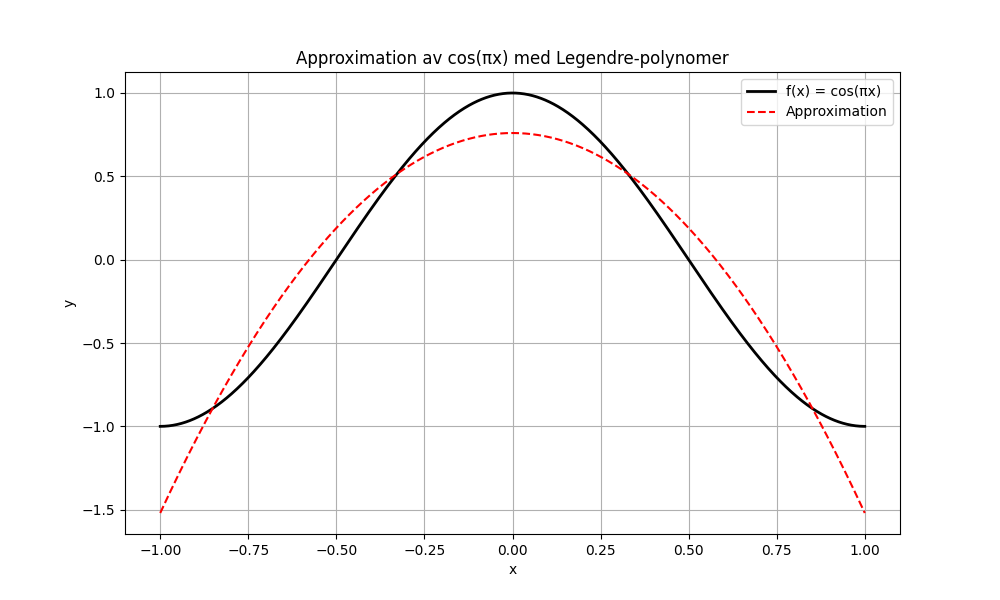
\includegraphics[width=0.9\textwidth,height=0.7\textheight,keepaspectratio]{figurer/Oppg_4.5.10c.png}
\end{center}
\end{proofbox}
\end{oppgavebox} 


\section*{4.7 Den adjungerte}
\addcontentsline{toc}{section}{4.7 Den adjungerte}


\begin{theorembox}{4.7.1}{}
for U og V endeligdimensjonale indreproduktrom over en kropp $ \mathbb{K} $, så er det en $ T \in \mathcal{L} \left( U, V \right)  $. da finnes en unik avbildning $ T^* \in \mathcal{L} \left( V, U \right) $ slik at \[
    \langle Tu, v \rangle_{ V } = \langle u, T^*v \rangle_{ U } \forall u\in U, v \in V 
\]

\end{theorembox}



  
\begin{oppgavebox}{4.7.3}{}
Vis også at $ \langle v, Tu \rangle_{ V } = \langle T^*v, u \rangle_{ U } \forall u\in U, v \in V $

\begin{proofbox}{4.7.3}{}
Skal vise at $ \langle v, Tu \rangle_{ V } = \langle T^*v, u \rangle_{ U }  \forall u \in U, v \in V$. Dette kan vises ved å benytte konjugert symmetri av indreprodukter

\begin{align*}
    \langle v, Tu \rangle_{ V } &= \overline{ \langle Tu, v \rangle_{ V } }\\
    &= \overline{ \langle u, T^*v \rangle_{ U }  } \\
    &= \langle T^*V, u \rangle_{ U }     
\end{align*}

\end{proofbox}
\end{oppgavebox}

\begin{oppgavebox}{4.7.4}{}
For tall $ a,b \in \mathbb{R} $, med $ a < b $  lar vi $ U:= C_0^{\infty} \left( \left[ a, b \right] \mathbb{R} \right)   $ der $ C_0^{\infty} \left\{ f \in C_0^0 \left( \left[ a, b \right], \mathbb{R} \right) : \frac{ d^n f }{ df^n } \in C_0^0 \left( \left[ a, b \right], \mathbb{R}  \right) \forall n \in \mathbb{N} \right\}  $


og der 
\[
    C_0^0 \left( \left[ a, b \right] , \mathbb{R} \right)  = \left\{ f \in C_0^0 \left( \left[ a, b \right] , \mathbb{R} \right): f(a) = f(b) = 0 \right\} 
\]

Dette rommet har indre prodiktet \[
    \langle f, g \rangle_{ U } = \int_{a}^{b} f(t) g(t) dt 
\]
La også $ T:U \rightarrow U$ være gitt ved $Tu =  \frac{ df }{ dt }$

\begin{itemize}
    \item a) Forklar hvorfor T er en veldefinert operator
    \item b) Selv om U ikke er endeligdimensjonal, så har T en adjungert finn denne
\end{itemize}


\begin{proofbox}{4.7.4 a)}{}
Siden T tar en kontinuerlig funksjon i U og spytter ut en annen funksjon i U, så må jeg vise at definisjonen av T er veldefinert, atlså $ Tf := \frac{ df }{ dt }$. Vi ser at U består av alle kontinuerlige funksjneoner som kan deriveres uendelig ganger. Det vil si at hvis vi deriverer den funksjonen en gang, så vil den deriverte fortsatt være i det samme rommet. Derfor kan vi si at T er veldefinert, fordi $ f, Tf $ er i det samme rommet. T er også lineær fordi derivering er lineær.
\end{proofbox}

\begin{proofbox}{4.7.4 b)}{}
Fra Riesz representasjonsteorem, så er det en unik $ u \in U $ slik at $ Sv = \langle v, u \rangle_{  }  $. Siden vi har at $ \langle f,g  \rangle_{  } = \int_{a}^{b} f(t)g(t) dt   $ så kan vi si at $ Sg = \int_{a}^{b} f(t) g(t) dt $

Den adjungerte til T er integrering
\end{proofbox}
\end{oppgavebox}

\begin{oppgavebox}{4.7.6}{}

\begin{itemize}
    \item ii) Vis at $ \left( T^* \right) ^*  =T $ 
    \item iv) Vis at om $ S \in \mathcal{L} \left( V, W \right)  $ så er $ \left( ST \right) ^* = T^* S^* $
    \item vi) $ imT^* = \left( ker T \right) ^{\bot} $

\end{itemize}

\begin{proofbox}{4.7.6 ii)}{}
    \begin{align*}
        \langle u, \left( T^* \right) ^* v \rangle_{  } &= \langle T^*u, v \rangle_{  } \\
        &= \overline{ \langle v, T^*u \rangle_{  } } \\
        &= \overline{ \langle Tv, u \rangle_{  }} \\
        &= \langle u, Tv \rangle_{  } 
    \end{align*} 
    Og jeg har vist at $ \left( T^* \right) ^*=T $ 
\end{proofbox}

\begin{proofbox}{4.7.6 iv)}{}
    \begin{align*}
        \langle u, \left( ST \right) ^* v \rangle_{  } &= \langle STu, v \rangle_{  } \\
        &= \overline{ \langle v, STu \rangle_{  } } \\
        &= \overline{ \langle S^* v, Tu \rangle_{  } } \\
        &= \overline{ \langle T^* S^* v, u \rangle_{  } } \\
        &= \langle u, T^* S^* v \rangle_{  } 
    \end{align*}
    Og jeg har vist at $ \left( ST \right) ^* = T^* S^* $ 
\end{proofbox}

\begin{proofbox}{4.7.6 vi)}{}
    Vi har at
    \begin{itemize}
        \item fra 4.5.7 i) at $ \left( V^{\bot} \right)^{\bot} = V  $ 
        \item fra 4.7.6 v) at $ ker T^* = \left( imT \right) ^{\bot} $
        \item fra 4.5.7 ii) at $ \left( T^* \right) ^* = T $   
    \end{itemize} 
    Dermed kan vi skrive 
    \begin{align*}
        imT &= \left( imT^{\bot} \right) ^{\bot} \\
        &= \left( ker T^* \right) ^{\bot}
    \end{align*}
    da vil 
    \begin{align*}
        imT^* &= \left( \left( T^* \right) ^* \right) ^{\bot} \\
        &= \left( kerT \right) ^{\bot}
    \end{align*}
\end{proofbox}
\end{oppgavebox}


\section*{4.8 Normale operatorer}
\addcontentsline{toc}{section}{4.8 Normale operatorer}


\begin{definitionbox}{4.8.1}{}
En operator T på et indreproduktrom er \textbf{\textit{normal}} hvis
$$
TT^* = T^*T
$$
En kvadratisk matrise $A \in M_n(\mathbb{K})$ er \textbf{\textit{normal}} hvis
$$
AA^* = A^*A
$$

der $A^* = \overline{A^T}$
\end{definitionbox}


\begin{oppgavebox}{4.8.2}{}
\begin{itemize}
    \item a) Vis at alle kvadratiske diagonal matriser er normale.
    \item b) Vis at alle unitære matriser er normale. En matrise er unitær om $ A^{-1} = A^* $
\end{itemize}

\begin{proofbox}{4.8.2 a)}{}
En kvadratisk matrise $ A \in M_n(\mathbb{K}) $ er normal hvis $ AA^* = A^*A $, der $ A^* $ er den konjugert-transponerte av $ A $.

Anta at $ A $ er en diagonal matrise, dvs. $ A = diag(\lambda_1, \lambda_2, \dots, \lambda_n) $. Da er:
\[
A = \begin{bmatrix}
\lambda_1 & 0 & \cdots & 0 \\
0 & \lambda_2 & \cdots & 0 \\
\vdots & \vdots & \ddots & \vdots \\
0 & 0 & \cdots & \lambda_n
\end{bmatrix}
\]

Den konjugert-transponerte matrisen $ A^* $ er:
\[
A^* = \begin{bmatrix}
\overline{\lambda_1} & 0 & \cdots & 0 \\
0 & \overline{\lambda_2} & \cdots & 0 \\
\vdots & \vdots & \ddots & \vdots \\
0 & 0 & \cdots & \overline{\lambda_n}
\end{bmatrix}
\]

Siden begge matrisene er diagonale, kommuterer de:
\[
AA^* = diag (|\lambda_1|^2, |\lambda_2|^2, \dots, |\lambda_n|^2) = A^*A
\]

Dermed er $ AA^* = A^*A $, og $ A $ er normal.
\end{proofbox}

\begin{proofbox}{4.8.2 b)}{}
    Anta at A er unitær. En matrise er normal om $ AA^* = A^*A $. Siden $ A^{-1}=A^* $, så er 
    \[
        A A^{-1} = I_n = A^{-1}A
    \]
    
\end{proofbox}
\end{oppgavebox}

\begin{oppgavebox}{4.8.3}{}

Vis at om T er normal, så er $ \left\lVert Tu \right\rVert = \left\lVert T^*u \right\rVert \forall u \in U $ 

\begin{proofbox}{4.8.3}{}
    Vi vet at $ \left\lVert Tu \right\rVert^2 =  \langle Tu, Tu \rangle_{  }  $ fra den normen indusert av indreproduktet. 

    \begin{align*}
        \langle Tu, Tu \rangle_{  }^2   &= \langle u, T^* Tu \rangle_{  }^2   \\
        &= \langle u, TT^* u \rangle_{  }^2\\
        &= \langle T^*u, T^*u \rangle_{  } \\
        &= \left\lVert T^*u \right\rVert ^2
    \end{align*}
\end{proofbox}

\end{oppgavebox}

\begin{oppgavebox}{4.8.4}{}
La $ U = C_0^{\infty} \left( \left[ a,b \right] , \mathbb{R} \right)  $ og la $ T \in \mathcal{L} \left( U \right)  $ være gitt ved $ Tf := \frac{ df }{ dt } $. Vis at T er normal
\begin{proofbox}{4.8.4}{}
La $ Tf := \frac{ df }{ dt } $ være som i oppgave 4.7.4. Da var $ T^* = \frac{ -df }{ dt } $

\begin{align*}
    T^*Tf &= - \frac{ d }{ dt }  \left( \frac{ df }{ dt } \right) \\
    &= - \frac{ d^2 f  }{ dt } \\
    &= \frac{ d }{ dt } \left( \frac{ -df }{ dt } \right) \\
    &= TT^*f
\end{align*}
\end{proofbox}


\end{oppgavebox}

\begin{theorembox}{4.8.5}{}
La T være en normal operator på et indreproduktrom U over $ \mathbb{K} $. Da gjelder
\begin{itemize}
    \item $ ker T = ker T^* $ 
    \item $ ker T = \left( imT \right)^{\bot}  $ 
    \item $ imT = imT^* $ 
    \item $ U = kerT \otimes im T$ 
    \item $ T - \alpha_{}^{} id   $  er normal for enhver $ \alpha_{}^{} \in \mathbb{K} $ 
\end{itemize}

\begin{proofbox}{4.8.5 iii) $ \to $ v)}{}
$ iii) \rightarrow v) $ Anta at $ imT = imT^* $. Skal vise at $ T - \alpha_{}^{} id $ er normal for enhver $ \alpha_{}^{} \in \mathbb{K} $ 

Sett $ S:= T - \alpha_{}^{} id $. Da er $ S^* = \left( T-\alpha_{}^{} id \right)  $ 

\begin{align*}
    SS^* &= \left( T-\alpha_{}^{} id \right) \left( T-\alpha_{}^{} id \right) ^* \\
    &= TT^* - T\overline{\alpha_{}^{} } - \alpha_{}^{} T + \alpha_{}^{} \overline{\alpha_{}^{} } \\
    &=T^*T - \overline{\alpha_{}^{} } T - T^* \alpha_{}^{} + \overline{\alpha_{}^{} } \alpha_{}^{}  \\
    &= \left( T-\alpha_{}^{} id \right) ^* \left( T- \alpha_{}^{} id \right) \\
    &= S^* S
\end{align*}
Så S er normal for alle $ \alpha_{}^{} \in \mathbb{K} $ 
\end{proofbox}

\end{theorembox}

\section*{4.9 Selvadjungerte operatorer}
\addcontentsline{toc}{section}{4.9 Selvadjungerte operatorer}


\begin{definitionbox}{4.9.1}{}
    En operator T på et indreproduktrom er selvadjungert om $ T = T^* $. En kvadratisk matrise $ A \in M_n(\mathbb{K}) $ er selvadjungert om $ A = A^* $ og er symmtrisk hvis $ A^T = A $ 
\end{definitionbox}

MERK: Over $ \mathbb{R} $ betyr selvadjungert og symmetrisk det samme


\begin{oppgavebox}{4.9.2}{}

a) Hvilke av de følgende matrisene er selvadjungerte?
\begin{enumerate}
    \item $ I_3 $
    \item $ 0_{4 \times 2} $  
    \item $ A = \begin{bmatrix}
        0&3i+1\\ i-3i& 2
    \end{bmatrix}  $ 
    \item $ B = \begin{bmatrix}
        7&1 \\ -1&7
    \end{bmatrix}  $ 
\end{enumerate}
b) Vis at alle selvadjungerte operatorer er normale

\begin{proofbox}{4.9.1}{}
\begin{itemize}
    \item for $ I_3 \in M_3(\mathbb{R}) $, som er kvadratisk, og symmetrisk fordi det er en diagonal matrise. Dermed er $ I_3 = I_3^* = I_3^T $  
    \item for $ 0_{4\times 2} \in M_{4 \times 2}(\mathbb{R}) $ som ikke er kvadratisk. Dermed er ikke $ 0_{4x2} = 0_{4 \times 2} = 0_{2 \times 4} = 0_{4 \times 2}^T $  
    \item for 
    \[
        A = \begin{bmatrix}
            0& 1-3i \\
            3i-1 & 2
        \end{bmatrix}  \in M_2(\mathbb{C})
    \]
    som ikke er med i relle tall, men er kvadratisk. $ A^* = \overline{A^T} $ 
    \[
        A_T = \begin{bmatrix}
            0& 1+3i\\
            3i-1&2
        \end{bmatrix} 
    \]
    dermed er \[
        \overline{A^T} = \begin{bmatrix}
            0&1+3i\\
            3i-1&2
        \end{bmatrix} \neq \begin{bmatrix}
            0&1+3i\\
            1-3i&2
        \end{bmatrix} 
    \]
    så $ A $ er ikke selv adjungert.
    \item for $ B = \begin{bmatrix}
        7&1\\
        -1&7
    \end{bmatrix} \in M_2(\mathbb{R}) $, så ser vi at 
    \[
        B^T = B^* = \begin{bmatrix}
            7&-1\\
            1&7
        \end{bmatrix} \neq \begin{bmatrix}
            7&1\\
            -1&7
        \end{bmatrix} =B
    \]
    Så B er ikke selv adjungert
\end{itemize}
\end{proofbox}

\begin{proofbox}{4.9.2 b)}{}
    Hvis T er selvadjungert så er $ T = T^* $. Og T er normal hvis $ TT^* = T^*T $. dvs. for en $ u \in U $, så er $ Tu = T^*u $. Med andre ord, så er 
    \[
        \langle Tu, T^*u \rangle_{  } =1
    \]
    Vi får da følgende:
    \begin{align*}
        \langle Tu, T^*u \rangle_{  } &= \langle u, T^*T^* u \rangle_{  } \\
        &= \langle TTu, u \rangle_{  } \\
        &= \overline{ \langle u, TTu \rangle_{  } }\\
        &= \overline{ \langle T^*T^*u, u \rangle_{  } } \\
        &= \langle u, T^*T^*u \rangle_{  } 
    \end{align*}
    Med andre ord, så må $ T=T^* $ hvis den er normal. Da har jeg vist at alle selvadjungerte matriser er normale. 
\end{proofbox}
\end{oppgavebox}

\section*{4.10 Ortogonale matriser og unitære operatorer} 
\addcontentsline{toc}{section}{4.10 Ortogonale matriser og unitære operatorer}


\begin{definitionbox}{4.10.1}{}
    La U være et endeligdim indreproduktrom. En operator T er \textbf{\textit{unitær}} om T er inverterbar, og $ T^{-1}=T^* $. En matrise $ A \in M_n(\mathbb{K}) $ er unitær om den er invertibel og $ A^{-1} = A^* $. Den er ortogonal om den er invertibel og $ A^T = A^{-1} $ 
\end{definitionbox}
MERK: Over $ \mathbb{R} $ betyr ortogonal og unitær det samme, men ikke over $ \mathbb{C} $ 


\begin{oppgavebox}{4.10.2}{}
La $ A \in M_n (\mathbb{K}) $. Forklar hvorfor følgende utsagn er ekvivalente:
\begin{itemize}
    \item A er unitær
    \item Kolonnene $ \left( a_1, ..., a_n \right)  $ er ortonormale
\end{itemize}
\begin{proofbox}{4.10.2}{}
    Om A er unitær, så er $ A^* = A^{-1} $. Det vil si at 
\[
    AA^* = I_n
\]
Dette sier altså at 
\[
\begin{cases}
\left( AA^* \right) _{ij} = 0 \text{ om } i \neq j \\
\left( AA^* \right) _{ij} = 1 \text{ om } i = j
\end{cases}
\] 

Dette forteller oss at $ \langle a_i, a_j \rangle_{  } =0 $ om $ i \neq j $, og $ \langle a_i, a_j \rangle_{  } = 1 $ om $ i=j $. Som er samme betingelse for at kolonnene $ \left( a_1, ..., a_n \right)  $ er ortonormale
\end{proofbox}
\end{oppgavebox}

\begin{propositionbox}{4.10.3}{}
La $ T \in \mathcal{L}(U) $.
\begin{itemize}
    \item T er normal
    \item $ T^* $ og $ T^{-1} $  er unitære
    \item for alle $ u \in U $ er
    \[
        \left\lVert Tu \right\rVert = \left\lVert T^{-1}u \right\rVert = \left\lVert T^* u \right\rVert = \left\lVert  u \right\rVert 
    \]
    \item $ T^{-1} $, $ T^* $ og T har alle operatornorm 1
    \item for alle $ R \in \mathcal{L}(U, V) $ og $ S \in \mathcal{L} (W, U) $ er 
    \[
        \left\lVert TS \right\rVert _{ \mathcal{L}} = \left\lVert S \right\rVert_{ \mathcal{L}} 
    \]
    og \[
        \left\lVert RT \right\rVert _{ \mathcal{L}}= \left\lVert R \right\rVert _{ \mathcal{L}}
    \]
    
        
      
\end{itemize} 
\end{propositionbox}

\begin{oppgavebox}{4.10.3}{}
\begin{proofbox}{4.10.3 i)}{}
    Siden T er unitær, så er $ T^* = T^{-1} $. Om T er normal, så er da $ TT^* = id  = TT^{-1} = id$ og åpenbart er da også $ T^{-1} T = id $ 
\end{proofbox}

ii)
\begin{proofbox}
    T er unitær om T er invertibel, og $ \left( ^* \right) ^* = \left( T^* \right) ^{-1} $ 

    Vet fra 4.7.6 ii) at $ \left( T^* \right) ^* = T $. I tillegg vet vi fra 4.7.6 iii) at hvis T er bijektiv, så er \[
        \left( T^* \right) ^{-1} = \left( T^{-1} \right) ^*
    \]
    Hvorfor er T bijektiv? 

    T er bijektiv om T er surjektiv og injektiv, altså at T er invertibel.
    Dermed vet vi at 
    \[
        \left( T^* \right) ^{-1} = \left( T^* \right) ^* = T
    \]
    Derfor er $ T^* ? T^{-1} $ og er av den grunn unitær 
\end{proofbox}

iii) For alle $ u \in U $ er 
\begin{align*}
    \left\lVert Tu \right\rVert &= \left\lVert u \right\rVert \\
    \left\lVert T^* u \right\rVert &= \left\lVert u \right\rVert \\
    \left\lVert T^{-1} \right\rVert &= \left\lVert u \right\rVert 
\end{align*}

\begin{proofbox}{4.10.3 iii) $ \left\lVert Tu \right\rVert = \left\lVert u \right\rVert  $ }{}
    Vet at \begin{align*}
        \left\lVert Tu \right\rVert ^2 &= \langle Tu, Tu \rangle_{  } ^2\\
        &= \langle u, T^*Tu \rangle_{  } ^2 \\
        &= \langle u, T^{-1}Tu \rangle_{  } ^2 \\
        &= \langle u, u \rangle_{  }^2\\
        &= \left\lVert u \right\rVert  ^2
    \end{align*}
\end{proofbox}

\begin{proofbox}{4.10.3 iii) $ \left\lVert T^{-1} u \right\rVert = \left\lVert u \right\rVert  $ }{}
    \begin{align*}
        \left\lVert T^{-1}u \right\rVert ^2 &= \langle T^{-1}u, T^{-1}u \rangle_{  } \\
        &= \langle u, \left( T^{-1} \right) *T^{-1}u \rangle_{  } ^2 \\
        &= \langle u, \left( T^* \right) ^*T^{-1}u \rangle_{  } ^2\\
        &= \langle u, u \rangle_{  }^2\\
        &= \left\lVert u \right\rVert  ^2
    \end{align*}
\end{proofbox}

\begin{proofbox}{4.10.3 iii) $ \left\lVert T^*u \right\rVert = \left\lVert u \right\rVert  $ }{}
    \begin{align*}
        \left\lVert T^*u \right\rVert ^2 &= \langle T^*u, T^*u \rangle_{  }^2 \\
        &= \langle u, \left( T^* \right) ^* T^*u \rangle_{  }  ^2 \\
        &= \langle u, TT^{-1}u \rangle_{  } ^2 \\
        &= \langle u, u \rangle_{  }^2\\
        &= \left\lVert u \right\rVert ^2 
    \end{align*}
\end{proofbox}
 

iv) $ T, T^*, T^{-1} $ har operator norm lik 1.

\begin{proofbox}{4.10.3 iv) $ T $ }{}
    \begin{align*}
        \left\lVert T \right\rVert &= sup_{u \in U, u \neq 0} \frac{ \left\lVert Tu \right\rVert  }{ \left\lVert u \right\rVert  }\\
        &= \frac{ \left\lVert u \right\rVert }{ \left\lVert u \right\rVert  }\\
        &= 1
    \end{align*}
\end{proofbox}

\begin{proofbox}{4.10.3 iv) $ T^* $ }{}
    \begin{align*}
        \left\lVert T^* \right\rVert &= sup_{u \in U, u \neq 0} \frac{ \left\lVert T^*u \right\rVert  }{ \left\lVert u \right\rVert  }\\
        &= \frac{ \left\lVert u \right\rVert }{ \left\lVert u \right\rVert  }\\
        &= 1
    \end{align*}
\end{proofbox}

\begin{proofbox}{4.10.3 iv) $ T^{-1} $ }{}
    \begin{align*}
        \left\lVert T^{-1} \right\rVert &= sup_{u \in U, u \neq 0} \frac{ \left\lVert T^{-1}u \right\rVert  }{ \left\lVert u \right\rVert  }\\
        &= \frac{ \left\lVert u \right\rVert }{ \left\lVert u \right\rVert  }\\
        &= 1
    \end{align*}
\end{proofbox}
\end{oppgavebox}


\begin{oppgavebox}{4.10.4}{}
La U være et indreprodukt rom med to ortonormale basiser $ \mathcal{B} = \left( u_1, ..., u_n \right)  $ og $ \mathcal{C} = \left( v_1, ..., v_n \right)  $. Vis at basisskiftematrisen $ \left[ id \right] _{ \mathcal{C}}^{ \mathcal{B}} $ er unitær.


\begin{proofbox}{4.10.4}{}
    Observerer først at 
    \[
        \langle u_i, u_j \rangle_{  } = \delta_{ij} 
    \] \[
        \langle v_i, v_j \rangle_{  } = \delta_{ij}
    \]
    Derfor er 
    \[
        I_n = \langle u_i, u_j \rangle_{  } = \delta_{ij} = \langle v_i, v_j \rangle_{  }
    \]
    Fra Def 2.6.2 vet vi at $ \left[ id \right] _{ \mathcal{B}}^{ \mathcal{C}} \left[ id \right] _{ \mathcal{B}}^{ \mathcal{C}} = I_n $. Dermed kan vi si at $ \left( \left[ id \right] _{ \mathcal{C}}^{ \mathcal{B}} \right)^* = \left[ id \right] _{ \mathcal{B}}^{ \mathcal{C}}  $  som betyr videre at $ \left( \left[ id \right] _{ \mathcal{C}}^{ \mathcal{B}} \right)^* = \left( \left[ id \right] _{ \mathcal{C}}^{ \mathcal{B}} \right)^{-1} $ som sier at $ \left[ id \right] _{ \mathcal{C}}^{ B} $ er unitær
\end{proofbox}
\end{oppgavebox}

\begin{oppgavebox}{4.10.7}{}
\begin{itemize}
    \item a) Hvor mange permutasjonsmatriser finnes av dimensjon $ n \times n $?
    \item b) Hva skjer med en vektor $ x \in \mathbb{K}^n $  når den ganges med en permutasjonsmatrise $ A \in M_n(\mathbb{K}) $ 
    \item c) Hva skjer med en matrise B om den ganges fra venstre med en permutasjonsmatrise? Hva om den ganges fra høyre?
\end{itemize}

\begin{proofbox}{4.10.7 a)}{}
En permutasjonsmatrise er en kvadratisk matrise slik at for hver rad og hver kolonne, så må summen

\[
    \sum_{ k=1 }^{ n } a_{jk} + \sum_{ j=1 }^{ n } a_{jk} = 1
\]
for $ j=1, ..., n $. Vet ikke om det er riktig formulert, men vil få frem at hvis vi plukker et element $ a_{jk} $ i en matrise som er slik at

\[
    A = \begin{bmatrix}
        1&0&0\\
        0&1_{jk}&0\\
        0&0&1
    \end{bmatrix} 
\]
hvor vi har plukket ut det jk te elementet. Anta også at $ A \in M_n(\mathbb{R}) $. Da kan ingen andre elementer $ a_{jk} $ for $ j=1,...n $ og samtidig for $ a_{jk} $ for $ k=1, ..., n $ være lik 1. Summen av den jte rad og den k te kolonnen må være lik 1, som forlater bare elementer $ a_{jk}=1 $.

For hver rad vi går gjennom, vil vi få en mindre plass og ha en 1 i for den neste raden. Dette fortsetter til vi kommer gjennom alle n radene. Og siden A er kvadratisk, så får vi $ n! $ forskjellige permutasjonsmatriser for en $ n \times  n$  matrisen $ A \in M_n(\mathbb{R}) $  

    
\end{proofbox}


\begin{proofbox}{4.10.7 b)}{}

Hvis du ganger en vektor $ x \in \mathbb{R}^n $ med en permutasjonsmatrise $ A \in M_n(\mathbb{R}) $ så vil du bare stokke om rekkefølgen på posisjonene til vektoren x. Dette skjer i forhold til hvilken plass i A som har en 1 i seg. Ta en vilkårlig matrise $ A $ med elementer $ a_{kj} $ og en vektor $ x = (x_k)_{k=1,...n} $. Da vil $ Ax $ bli den nye vektoren, bare at $ x_k $ og $ x_j $ (fordi $ A\in M_n(\mathbb{R}) $ og $ x \in \mathbb{R}^n $  ) bytter om element.

Ta for eksempel $ A = \begin{bmatrix}
    1&0&0\\
    0&0&1\\
    0&1&0
\end{bmatrix}  $ og $ x = \begin{bmatrix}
    x_1\\
    x_2\\
    x_3
\end{bmatrix}  $ 
Da vil $ Ax = \begin{bmatrix}
    x_1\\
    x_3\\
    x_2
\end{bmatrix}  $ 
    
\end{proofbox}

\begin{proofbox}{4.10.7 c)}{}
Om vi ganger en kvadratisk matrise B med en permutasjonsmatrise fra venstre, så vil rad nr j og k bytte plass, om det er en 1 i posisjon $ a_{jk} $  i permutasjonsmatrisen A

Om vi ganger en kvadratisk matrise B med en permutasjonsmatrise fra høyre side, så vil kolonnene j og k bytte plass, om det er en 1 i posisjon $ a_{jk} $ i permutasjonsmatrisen  
\end{proofbox}

\end{oppgavebox}

\section*{4.11 Triangulære matriser, LU og QR faktorisering}
\addcontentsline{toc}{section}{4.11 Triangulære matriser, LU og QR faktorisering}

\begin{oppgavebox}{4.11.3}{}
La A ha LU faktorisering og betrakt systemet $ Ax=b $. Vis at dersom y løser $ Ly=b $ så løse x $ Ux = y $

\begin{proofbox}{4.11.3}{}
    \begin{align*}
        Ax &= b \\
        LUx &= b\\
        L \left( Ux \right) &= b\\
        Ly &= b \\
    \end{align*}
    og det er vist.
\end{proofbox}
\end{oppgavebox}

\end{document}